\clearpage
\section{边界条件建模}
\label{chap:boundary-conditions-modelling}
\renewcommand{\thestatement}{1.\arabic{statement}}
\renewcommand{\theHstatement}{ch07.sec01.\arabic{statement}}
\setcounter{statement}{0}
\setcounter{figure}{0}
\renewcommand{\thefigure}{VII.\arabic{figure}}
\newcounter{chaptersevensectiononeremark}
\renewcommand{\thechaptersevensectiononeremark}{1.\arabic{chaptersevensectiononeremark}}
\begin{sloppypar}

本章考虑在计算实际流动的数值近似时可能遇到的两类不同边界条件问题. 当计算区域并不恰好等于所关注的原始物理区域时, 就会出现这些问题.

\begin{itemize}
 \item 在 Section~\ref{sec:chap7-outflow-boundary-conditions} 中, 考虑计算区域严格小于物理区域的情形 (例如为了节省计算资源, 或者因为物理区域无界). 因此, 必须在边界的非物理部分提出人工边界条件, 并分析所得系统. 我们讨论这样的流动: 速度在边界的一部分上给定, 而在另一部分上可以自由流出. 这种情形的一个例子是管网, 其中输入速度在管网的若干位置上给定, 但在输出端仍然未知.

 从数学和数值观点看, 必须在边界的流出部分选择边界条件. 本节提出一个非线性边界条件, 其目标是为 Navier--Stokes 方程提供一个稳定解, 并希望该解足够接近真实流动.
 \item 反过来, 在 Section~\MBUnresolvedReference{sec:chap7-dirichlet-penalty}{2} 中, 考虑计算区域大于物理区域的情形. 这称为虚拟区域方法. 当希望避免非结构网格或移动网格上的数值方法所带来的困难时, 常会采用这种方法. 我们把计算区域中不属于物理区域的部分称为障碍物.

 本节关注如何用罚方法在真实物理边界上考虑 Navier--Stokes 方程的 Dirichlet 边界条件. 这种方法在障碍物内部的方程中加入某个非物理项, 其作用是考虑障碍物边界上的真实边界条件. 我们证明该近似是适定的, 并分析当罚参数趋于 $0$ 时它向真实解的收敛性.
\end{itemize}

除了这两个问题各自在实际情形中的特殊意义之外, 它们还使我们有机会介绍一些在许多其他框架中也可能有用的数学方法.

\subsection{流出边界条件}
\label{sec:chap7-outflow-boundary-conditions}

一般而言, 无论遇到何种物理情形, 当我们希望计算物体周围的流动时 (例如机翼周围气流这一经典情形), 都必须或多或少任意地截断物理区域, 以得到一个合适的计算区域. 此时, 在区域的``非物理''边界上写出真实的边界条件是有用的, 从而得到数学上适定并且能够描述所研究物理情形的问题.

典型地, 当 Reynolds 数很高而流动不再是层流时, 在流动出口处 (即流体平均而言离开计算区域的位置) 会产生湍流结构. 尽管净流量向外, 速度场却交替地流出和重新流入区域. 然而, 在速度场离开区域的位置, 可以直观地理解为没有必要施加边界条件; 相反, 在速度场进入区域的位置, 则绝对有必要给出某个边界条件.

为处理这一困难, 我们描述流动下游的弱反射边界条件, 也就是说, 这种边界条件不会使系统能量增加过多. 这些边界条件最初在文献\MBUnresolvedReference{bib:outflow-boundary-original}{[29, 30]}中提出并研究. 文献\MBUnresolvedReference{bib:nonhomogeneous-outflow}{[25]}把这些结果推广到了非齐次 Navier--Stokes 方程的情形.

\subsubsection{模型的建立}
\label{subsec:chap7-outflow-model}

设 $\Omega$ 是 $\mathbb R^d$ 中的有界 Lipschitz 区域, 其中 $d=2$ 或 $d=3$. 记其边界为 $\Gamma=\partial\Omega$, 并考虑 $\Gamma$ 的分解
\[
 \Gamma=\Gamma_1\cup\Gamma_2,
\]
其中 $\Gamma_1$ 和 $\Gamma_2$ 的表面测度均非零. 假设 Dirichlet 边界数据 $g_1$ 在 $\Gamma_1$ 上已知 ($\Gamma_1$ 表示流动的上游部分), 并考虑如下问题: 寻找二元组 $(v,p)$, 使其满足
\begin{equation}
\left\{
\begin{aligned}
 \frac{\partial v}{\partial t}+(v\cdot\nabla)v-\operatorname{div}\sigma(v,p)&=0&&\text{于 }\Omega,\\
 \operatorname{div}v&=0&&\text{于 }\Omega,\\
 v&=g_1&&\text{于 }\Gamma_1,\\
 v(0)&=v_0,
\end{aligned}
\right.
\label{eq:chap7-outflow-navier-stokes-problem}
\end{equation}
其中
\[
 \sigma(v,p)=\frac2{\operatorname{Re}}D(v)-p\operatorname{Id}
\]
是流动的应力张量, 应变率张量定义为
\[
 D(v)=\frac12(\nabla v+{}^t\nabla v).
\]

还必须在 $\Gamma_2$ 上给出一个边界条件 (所建模的物理情形并未规定这一条件), 以尽可能精确地考虑没有计算的流动下游部分, 见 Figure~\ref{fig:chap7-truncated-physical-domain}. 显然, 这个边界条件必须与流动经过 $\Gamma_2$ 时所受的应力有关. 暂时可将它写成一般形式
\begin{equation}
 \sigma(v,p)\cdot\nu=F(v),
 \qquad\text{于 }\Gamma_2,
\label{eq:chap7-general-outflow-condition}
\end{equation}
其中函数 $F$ 将在下文规定.

\begin{figure}[H]
\centering
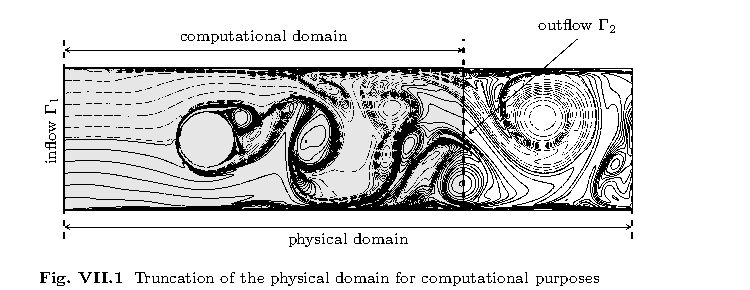
\includegraphics[width=.82\textwidth,trim=0 30bp 0 0,clip]{figures/ch07-fig01.png}
\caption{为计算目的对物理区域进行截断.}
\label{fig:chap7-truncated-physical-domain}
\end{figure}

为了构造所考虑的边界条件, 需要选取某个参考流 $u_{\mathrm{ref}}$, 它是满足
\[
 u_{\mathrm{ref}}\in(H^1(\Omega))^d,
 \qquad u_{\mathrm{ref}}=g_1\quad\text{于 }\Gamma_1
\]
的任意函数. 为了使方法有效, 重要的是选择 $u_{\mathrm{ref}}$, 使其在 $\Gamma_2$ 附近合理地逼近预期流动 (当然该流动是未知的).

为简化计算, 尽管这完全不是必要的, 假设 $u_{\mathrm{ref}}$ 是如下欠定稳态 Stokes 问题的一个解:
\begin{equation}
\left\{
\begin{aligned}
 -\operatorname{div}\sigma(u_{\mathrm{ref}},p_{\mathrm{ref}})
 =-\frac1{\operatorname{Re}}\Delta u_{\mathrm{ref}}+\nabla p_{\mathrm{ref}}&=0&&\text{于 }\Omega,\\
 \operatorname{div}u_{\mathrm{ref}}&=0&&\text{于 }\Omega,\\
 u_{\mathrm{ref}}&=g_1&&\text{于 }\Gamma_1.
\end{aligned}
\right.
\label{eq:chap7-reference-stokes-problem}
\end{equation}
还需要在边界的流出部分 $\Gamma_2$ 上选择参考应力张量 $\sigma_{\mathrm{ref}}$. 这里同样为了略微简化, 直接选择
\begin{equation}
 \sigma_{\mathrm{ref}}\cdot\nu
 =\sigma(u_{\mathrm{ref}},p_{\mathrm{ref}})\cdot\nu
 \in(H^{-1/2}(\partial\Omega))^d.
\label{eq:chap7-reference-stress}
\end{equation}
从现在起, 假设 $u_{\mathrm{ref}}$ 和 $\sigma_{\mathrm{ref}}$ 已固定且与时间无关.

于是寻找形如 $(v=u+u_{\mathrm{ref}},p)$ 的问题\eqref{eq:chap7-outflow-navier-stokes-problem}之解, 其中 $u$ 在 $\Gamma_1$ 上满足齐次边界条件, 而 $\Gamma_2$ 上的条件以弱意义满足.

引入与该问题自然相联系的函数空间
\[
 V=\{\varphi\in(H^1(\Omega))^d:\varphi|_{\Gamma_1}=0,
 \ \operatorname{div}\varphi=0\},
\]
\[
 H=\overline V^{(L^2(\Omega))^d},
\]
即 $V$ 在 $(L^2(\Omega))^d$ 中的闭包. 注意, 由于 Dirichlet 边界条件只在 $\Gamma_1$ 上给定, 这些空间不同于 Chapter~\ref{chap:steady-stokes-equations} Section~\ref{subsec:chap4-leray-decomposition} 中引入的空间 $V$ 和 $H$. 因此, 寻找二元组 $(u,p)$, 其中几乎每个 $t$ 都有 $u(t)\in V$, 并且二元组 $(u+u_{\mathrm{ref}},p)$ 对任意 $\psi\in V$ 满足问题\eqref{eq:chap7-outflow-navier-stokes-problem}的如下弱形式:
\[
\begin{aligned}
 &\frac{\mathrm d}{\mathrm dt}\int_\Omega(u+u_{\mathrm{ref}})\cdot\psi\,\mathrm dx
 +\int_\Omega\sigma(u+u_{\mathrm{ref}},p+p_{\mathrm{ref}}):\nabla\psi\,\mathrm dx\\
 &\quad+\frac12\int_\Omega\Bigl[
 (((u+u_{\mathrm{ref}})\cdot\nabla)(u+u_{\mathrm{ref}}))\cdot\psi
 -(((u+u_{\mathrm{ref}})\cdot\nabla)\psi)\cdot(u+u_{\mathrm{ref}})
 \Bigr],\mathrm dx\\
 &=-\frac12\int_{\Gamma_2}((u+u_{\mathrm{ref}})\cdot\psi)
 ((u+u_{\mathrm{ref}})\cdot\nu)\,\mathrm d\sigma
 +\langle\sigma(u+u_{\mathrm{ref}},p+p_{\mathrm{ref}})\cdot\nu,
 \psi\rangle_{H^{-1/2},H^{1/2}}.
\end{aligned}
\]
这个方程当然理解为 $]0,T[$ 上的分布等式. 与 Chapter~\ref{chap:homogeneous-navier-stokes} 中一样, 可以写出采用依赖于时间的测试函数的弱形式. 此外, 可以在该形式中加入以 $V'$ 的弱意义满足的初始数据.

这一形式考虑了 $\Gamma_1$ 上的非齐次 Dirichlet 边界条件以及 $u_{\mathrm{ref}}$ 是该边界条件的提升这一事实. 现在需要详细说明 $\Gamma_2$ 上施加的条件. 思路如下. 在流动向外的位置 (即 $v\cdot\nu=(u+u_{\mathrm{ref}})\cdot\nu>0$ 时), 对流体施加来自所选参考流 (一般为非湍流流动) 的约束. 相反, 若 $v\cdot\nu=(u+u_{\mathrm{ref}})\cdot\nu<0$, 为了稳定性, 就必须控制惯性通过边界所产生的能量增长. 换言之, 在 $(u+u_{\mathrm{ref}})\cdot\nu<0$ 的情形下, 必须考虑位于计算区域之外 ($\Gamma_2$ 的另一侧) 的流体所施加的压力, 而对该流体当然一无所知. 回顾速度场范数的平方与压力除以密度之商具有相同的齐次性, 可知必须在 $\Gamma_2$ 上加入的约束项应当二次依赖于速度.

为同时考虑两种情形 (即边界的流入部分和流出部分), 把边界条件\eqref{eq:chap7-general-outflow-condition}规定为
\begin{equation}
 \sigma(u+u_{\mathrm{ref}},p+p_{\mathrm{ref}})\cdot\nu
 =-\frac12((u+u_{\mathrm{ref}})\cdot\nu)^-u
 +\sigma_{\mathrm{ref}}\cdot\nu,
 \qquad\text{于 }\Gamma_2.
\label{eq:chap7-nonlinear-outflow-condition}
\end{equation}
回顾任意实数的正部和负部定义于 Definition~\ref{def:chap6-positive-negative-parts}.

下面说明, \eqref{eq:chap7-nonlinear-outflow-condition}中二次项的选择恰好能够补偿边界非物理部分上的惯性项贡献所含的能量, 在该处流体正在进入区域.

\par\noindent\refstepcounter{chaptersevensectiononeremark}\textbf{Remark~\thechaptersevensectiononeremark:}\label{rem:chap7-reference-outflow-condition}
\begin{itemize}
 \item 文献\MBUnresolvedReference{bib:alternative-outflow-boundaries}{[30]}中可以找到这类其他边界条件. 此外注意, 这些边界条件实际上依赖于参考流 $u_{\mathrm{ref}},\sigma_{\mathrm{ref}}$.

 从物理和数值观点看, 选择一个``良好''参考流显然至关重要. 事实上, 若碰巧 $v=u_{\mathrm{ref}}$, 即 $u=0$, 则\eqref{eq:chap7-nonlinear-outflow-condition}恰好成立. 因此, 若能先验地选择与预期解相差不大的 $(u_{\mathrm{ref}},\sigma_{\mathrm{ref}})$, 那么计算所得的解将接近精确流动. 这当然依赖于所研究的物理情形.
 \item 文献\MBUnresolvedReference{bib:nonhomogeneous-outflow}{[25]}研究了不可压缩非齐次流动情形下的同类边界条件 (即 Chapter~\ref{chap:nonhomogeneous-fluids} 中研究的同一模型). 特别地, 其中证明 $\sigma_{\mathrm{ref}}$ 和 $u_{\mathrm{ref}}$ 不必由关系\eqref{eq:chap7-reference-stress}联系, 并且还可以依赖于时间.
\end{itemize}

把边界条件\eqref{eq:chap7-nonlinear-outflow-condition}代入问题, 并利用 $u_{\mathrm{ref}}$ 是稳态 Stokes 问题\eqref{eq:chap7-reference-stokes-problem}的解这一事实, 则现在所研究的弱形式对任意测试函数 $\psi\in V$ 可写为
\[
\begin{aligned}
 &\frac{\mathrm d}{\mathrm dt}\int_\Omega u\cdot\psi\,\mathrm dx
 +\int_\Omega\sigma(u,p):\nabla\psi\,\mathrm dx\\
 &\quad+\frac12\int_\Omega\Bigl[
 (((u+u_{\mathrm{ref}})\cdot\nabla)(u+u_{\mathrm{ref}}))\cdot\psi
 -(((u+u_{\mathrm{ref}})\cdot\nabla)\psi)\cdot(u+u_{\mathrm{ref}})
 \Bigr],\mathrm dx\\
 &\quad+\frac12\int_{\Gamma_2}(u\cdot\psi)
 ((u+u_{\mathrm{ref}})\cdot\nu)^+,\mathrm d\sigma
 =-\frac12\int_{\Gamma_2}(u_{\mathrm{ref}}\cdot\psi)
 ((u+u_{\mathrm{ref}})\cdot\nu)^-,\mathrm d\sigma.
\end{aligned}
\]
利用对称张量与反对称张量的双重缩并乘积为零这一事实, 对任意 $\psi\in V$ 有
\[
\begin{aligned}
 \sigma(u,p):\nabla\psi
 &=\frac2{\operatorname{Re}}D(u):
 \left(D(\psi)+\frac12(\nabla\psi-{}^t\nabla\psi)\right)
 -p\operatorname{div}\psi\\
 &=\frac2{\operatorname{Re}}D(u):D(\psi).
\end{aligned}
\]
最终, 关于 $u$ 的弱形式不再显式含有压力项, 因而问题化为寻找映射 $t\mapsto u(t)\in V$, 使其对任意 $\psi\in V$ 在 $\mathcal D'(]0,T[)$ 中满足
\begin{equation}
\begin{aligned}
 &\frac{\mathrm d}{\mathrm dt}\int_\Omega u\cdot\psi\,\mathrm dx
 +\frac2{\operatorname{Re}}\int_\Omega D(u):D(\psi)\,\mathrm dx\\
 &\quad+\frac12\int_\Omega\Bigl[
 (((u+u_{\mathrm{ref}})\cdot\nabla)(u+u_{\mathrm{ref}}))\cdot\psi
 -(((u+u_{\mathrm{ref}})\cdot\nabla)\psi)\cdot(u+u_{\mathrm{ref}})
 \Bigr],\mathrm dx\\
 &\quad+\frac12\int_{\Gamma_2}(u\cdot\psi)
 ((u+u_{\mathrm{ref}})\cdot\nu)^+,\mathrm d\sigma
 =-\frac12\int_{\Gamma_2}(u_{\mathrm{ref}}\cdot\psi)
 ((u+u_{\mathrm{ref}})\cdot\nu)^-,\mathrm d\sigma.
\end{aligned}
\label{eq:chap7-outflow-weak-formulation}
\end{equation}

\subsubsection{存在性与唯一性}
\label{subsec:chap7-outflow-existence-uniqueness}

本小节证明如下结果.

\begin{Theorem}
\label{thm:chap7-outflow-existence-uniqueness}
设 $\Omega$ 是 $\mathbb R^d$ 中连通的有界 Lipschitz 区域, $d\in\{2,3\}$. 设 $\operatorname{Re}>0$, $g_1\in(H^{1/2}(\Gamma))^d$, 且 $(u_{\mathrm{ref}},p_{\mathrm{ref}})$ 是\eqref{eq:chap7-reference-stokes-problem}的唯一解.

对任意 $v_0\in u_{\mathrm{ref}}+H$ 和任意 $T>0$, 至少存在一个
\[
 u\in L^\infty(]0,T[,H)\cap L^2(]0,T[,V)
\]
是\eqref{eq:chap7-outflow-weak-formulation}的解, 并且对任意 $\psi\in V$ 有
\begin{equation}
 \left(\int_\Omega u\cdot\psi\,\mathrm dx\right)(0)
 =\int_\Omega u_0\cdot\psi\,\mathrm dx,
 \qquad u_0=v_0-u_{\mathrm{ref}}.
\label{eq:chap7-outflow-initial-condition}
\end{equation}
此外,
\[
 \frac{\mathrm du}{\mathrm dt}\in L^{4/d}(]0,T[,V'),
\]
并且该解在维数 $d=2$ 时唯一.

最后, 存在 $p\in W^{-1,\infty}(]0,T[,L_0^2(\Omega))$, 使二元组 $(v=u_{\mathrm{ref}}+u,p)$ 是 $\Omega$ 中 Navier--Stokes 方程的解.
\end{Theorem}

初始条件\eqref{eq:chap7-outflow-initial-condition}有意义, 因为对\eqref{eq:chap7-outflow-weak-formulation}的任意解, 利用 Corollary~\ref{cor:chap2-w11-continuous-representative}可知
\[
 t\longmapsto\int_\Omega u\cdot\psi\,\mathrm dx
\]
关于时间连续.

\paragraph{近似问题的定义}
\label{subsec:chap7-outflow-approximate-problem}

回到上面引入的函数空间 $V$. 该空间是 $(H^1(\Omega))^d$ 的闭子空间, 因而特别是一个可分 Hilbert 空间. 所以它具有一组可数 Hilbert 基 $(w_k)_k$.

构造适合弱形式\eqref{eq:chap7-outflow-weak-formulation}的近似问题. 令 $H_N$ 是函数 $(w_k)_{k\leq N}$ 张成的向量空间. 考虑如下 Galerkin 逼近: 寻找映射 $t\mapsto u_N(t)\in H_N$, 使其对任意 $\psi\in H_N$ 满足
\begin{equation}
\begin{aligned}
 &\frac{\mathrm d}{\mathrm dt}\int_\Omega u_N\cdot\psi\,\mathrm dx
 +\frac2{\operatorname{Re}}\int_\Omega D(u_N):D(\psi)\,\mathrm dx\\
 &\quad+\frac12\int_\Omega\Bigl[
 (((u_N+u_{\mathrm{ref}})\cdot\nabla)(u_N+u_{\mathrm{ref}}))\cdot\psi
 -(((u_N+u_{\mathrm{ref}})\cdot\nabla)\psi)\cdot(u_N+u_{\mathrm{ref}})
 \Bigr],\mathrm dx\\
 &\quad+\frac12\int_{\Gamma_2}(u_N\cdot\psi)
 ((u_N+u_{\mathrm{ref}})\cdot\nu)^+,\mathrm d\sigma
 =-\frac12\int_{\Gamma_2}(u_{\mathrm{ref}}\cdot\psi)
 ((u_N+u_{\mathrm{ref}})\cdot\nu)^-,\mathrm d\sigma.
\end{aligned}
\label{eq:chap7-outflow-galerkin-problem}
\end{equation}

在此不采用由某个适当算子的特征函数构造的特殊基, 这与 Chapter~\ref{chap:homogeneous-navier-stokes} 中的方法不同. 原因是, 研究在 $\Gamma_1$ 上为 Dirichlet 型而在 $\Gamma_2$ 上为 Neumann 型的混合边界条件下的 Stokes 算子会带来一些这里不想处理的额外困难.

正因为如此, 不能先验地知道函数 $w_k$ 是正则的; 此外, 也不知道如何估计正交投影 $P_N:H\to H_N\subset H$ 在 $V$ 中被视为 (非正交) 投影时的范数. 因此, 不能像 Chapter~\ref{chap:homogeneous-navier-stokes} 的 Lemma~\ref{lem:chap5-galerkin-time-derivative} 中那样得到近似解时间导数的估计.

为此, 这里以关于时间的分数阶导数估计代替 $\mathrm du_N/\mathrm dt$ 的估计. 该估计利用 Chapter~\ref{chap:analysis-tools} Section~\ref{subsec:chap2-banach-fourier} 中引入的时间 Fourier 变换得到. 利用 Proposition~\ref{prop:chap2-fourier-nikolskii}, 可以在一个适当选取的 Nikolskii 空间中估计近似解. 这足以得到所需的紧性性质 (见 Theorem~\ref{thm:chap2-simon-nikolskii-compactness}).

文献\MBUnresolvedReference{bib:dirichlet-fourier-compactness}{[84]}对通常 Dirichlet 边界条件下的 Navier--Stokes 方程详细描述了这一一般方法.

\paragraph{能量不等式}
\label{subsec:chap7-outflow-energy-inequality}

\begin{Proposition}
\label{prop:chap7-outflow-galerkin-energy}
近似系统\eqref{eq:chap7-outflow-galerkin-problem}在 $\mathbb R^+$ 上有唯一整体解, 且对任意 $T>0$, 存在与 $N$ 无关的常数 $C$, 使
\begin{equation}
\begin{aligned}
 &\sup_{t\leq T}\|u_N(t)\|_{L^2}^2
 +\frac1{\operatorname{Re}}\int_0^T\|\nabla u_N(t)\|_{L^2}^2\,\mathrm dt\\
 &\qquad+\int_0^T\int_{\Gamma_2}|u_N|^2
 ((u_N+u_{\mathrm{ref}})\cdot\nu)^+,\mathrm d\sigma\,\mathrm dt
 \leq C.
\end{aligned}
\label{eq:chap7-outflow-uniform-energy}
\end{equation}
\end{Proposition}

\begin{Proof}
按照通常方法, 方程\eqref{eq:chap7-outflow-galerkin-problem}等价于一个有限维常微分方程组. Cauchy--Lipschitz Theorem 给出该系统在最大时间区间 $[0,T_N[$ 上解的存在唯一性. 为了证明解是整体的并得到估计\eqref{eq:chap7-outflow-uniform-energy}, 现在只需建立具有与 $N$ 无关界的能量不等式.

取 $\psi=u_N(t)=(u_N(t)+u_{\mathrm{ref}})-u_{\mathrm{ref}}$ 为测试函数, 并注意 $\psi$ 对时间的依赖, 得
\[
\begin{aligned}
 &\frac12\frac{\mathrm d}{\mathrm dt}\|u_N\|_{L^2}^2
 +\frac2{\operatorname{Re}}\|D(u_N)\|_{L^2}^2
 +\frac12\int_{\Gamma_2}|u_N|^2
 ((u_N+u_{\mathrm{ref}})\cdot\nu)^+,\mathrm d\sigma\\
 &\leq\left|\int_\Omega
 (((u_N+u_{\mathrm{ref}})\cdot\nabla)u_N)\cdot u_{\mathrm{ref}}
 -(((u_N+u_{\mathrm{ref}})\cdot\nabla)u_{\mathrm{ref}})\cdot u_N
 \,\mathrm dx\right|\\
 &\quad+\frac12\left|\int_{\Gamma_2}(u_N\cdot u_{\mathrm{ref}})
 ((u_N+u_{\mathrm{ref}})\cdot\nu)^-,\mathrm d\sigma\right|\\
 &\leq\|u_N+u_{\mathrm{ref}}\|_{L^3}
 \bigl(\|\nabla u_N\|_{L^2}\|u_{\mathrm{ref}}\|_{L^6}
 +\|u_N\|_{L^6}\|\nabla u_{\mathrm{ref}}\|_{L^2}\bigr)\\
 &\quad+\|u_N+u_{\mathrm{ref}}\|_{L^{8/3}(\Gamma_2)}
 \|u_N\|_{L^{8/3}(\Gamma_2)}
 \|u_{\mathrm{ref}}\|_{L^4(\Gamma_2)}.
\end{aligned}
\]
由 Sobolev 不等式 Proposition~\ref{prop:chap3-gagliardo-nirenberg-interpolation},
\[
 \|u_N\|_{L^3}\leq C\|u_N\|_{L^2}^{1/2}
 \|\nabla u_N\|_{L^2}^{1/2}.
\]
又有 $\|u_N\|_{L^{8/3}(\Gamma_2)}\leq\|u_N\|_{L^{8/3}(\Gamma)}$, 因而由 Theorem~\ref{thm:chap3-boundary-sobolev-embedding}和广义 Poincaré 不等式 Proposition~\ref{prop:chap3-generalized-poincare},
\[
 \|u_N\|_{L^{8/3}(\Gamma_2)}
 \leq C\|u_N\|_{L^2}^{1/4}\|\nabla u_N\|_{L^2}^{3/4}.
\]
注意这些不等式在维数 $2$ 和维数 $3$ 下都成立. 还回顾 $u_{\mathrm{ref}}$ 是 $(H^1(\Omega))^d$ 中固定的参考稳态流. 因此存在仅依赖于 $u_{\mathrm{ref}}$ 和 $\Omega$ 的常数 $C>0$, 使
\[
\begin{aligned}
 &\frac12\frac{\mathrm d}{\mathrm dt}\|u_N\|_{L^2}^2
 +\frac2{\operatorname{Re}}\|D(u_N)\|_{L^2}^2
 +\frac12\int_{\Gamma_2}|u_N|^2
 ((u_N+u_{\mathrm{ref}})\cdot\nu)^+,\mathrm d\sigma\\
 &\qquad\leq C\left(1+\|\nabla u_N\|_{L^2}
 +\|u_N\|_{L^2}^{1/2}\|\nabla u_N\|_{L^2}^{3/2}\right).
\end{aligned}
\]
现在必须用 Korn 不等式 Lemma~\ref{lem:chap4-korn-inequality}, 以 $\|D(u_N)\|$ 控制 $\|\nabla u_N\|$. 因而适当使用 Young 不等式得到
\[
\begin{aligned}
 &\frac12\frac{\mathrm d}{\mathrm dt}\|u_N\|_{L^2}^2
 +\frac1{\operatorname{Re}}\|D(u_N)\|_{L^2}^2
 +\frac12\int_{\Gamma_2}|u_N|^2
 ((u_N+u_{\mathrm{ref}})\cdot\nu)^+,\mathrm d\sigma\\
 &\qquad\leq\frac1{\operatorname{Re}}\|D(u_N)\|_{L^2}^2
 +C(1+\|u_N\|_{L^2}^2),
\end{aligned}
\]
其中 $C$ 依赖于 $u_{\mathrm{ref}}$. 由 Gronwall Lemma, 存在与 $N$ 无关的 $C(T)>0$, 使
\[
\begin{aligned}
 &\sup_{t\leq T}\|u_N(t)\|_{L^2}^2
 +\frac1{\operatorname{Re}}\int_0^T\|D(u_N)\|_{L^2}^2\,\mathrm dt\\
 &\qquad+\int_0^T\int_{\Gamma_2}|u_N|^2
 ((u_N+u_{\mathrm{ref}})\cdot\nu)^+,\mathrm d\sigma\,\mathrm dt
 \leq C(T).
\end{aligned}
\]
最后再次使用 Korn 不等式即得到所需不等式\eqref{eq:chap7-outflow-uniform-energy}.
\end{Proof}

与 Chapter~\ref{chap:homogeneous-navier-stokes} 中一样, 由上述估计推出经 Galerkin 方法得到的近似解在 $\mathbb R^+$ 上整体存在, 即存在时间 $T_N=+\infty$.

\par\noindent\refstepcounter{chaptersevensectiononeremark}\textbf{Remark~\thechaptersevensectiononeremark:}\label{rem:chap7-quadratic-boundary-optimality}
对于 $\mathbb R^3$ 中光滑有界区域 $\Omega$, $s>0$ 时族 $H^s(\Gamma)$ 中能够嵌入 $L^3(\Gamma)$ 的最大边界 Sobolev 空间是 $H^{1/3}(\Gamma)$ (因为 $\Gamma$ 是二维流形). 这是与分数阶 Sobolev 空间 $H^{5/6}(\Omega)$ 相联系的迹空间, 因为 $1/3=5/6-1/2$. 利用 Sobolev 嵌入和插值 (Theorem~\ref{thm:chap2-mixed-lp-interpolation}), 得到 $L^\infty(]0,T[,L^2(\Omega))\cap L^2(]0,T[,H^1(\Omega))$ 中的函数只属于 $L^{12/5}(]0,T[,H^{5/6}(\Omega))$. 因而 $|u|^3$ 在 $]0,T[\times\Gamma$ 上不可积, 因为它关于时间不够正则. 从数学观点看, 这说明流出边界条件必须是二次的, 才能得到适定系统.

\paragraph{关于时间的分数阶导数估计}
\label{subsec:chap7-outflow-fractional-time-estimate}

为了利用紧性定理在非线性项中取极限, 现在需要得到速度 $u_N$ 的一个附加估计. 这里采用关于时间的分数阶导数, 更准确地说, 采用时间变量的 Fourier 变换; Chapter~\ref{chap:analysis-tools} Section~\ref{subsec:chap2-banach-fourier} 中已经详细说明其性质. 重新使用记号 $\widetilde u_N$ 表示 $u_N$ 在整个时间区间 $\mathbb R$ 上的零延拓.

\begin{Proposition}
\label{prop:chap7-outflow-fourier-estimate}
对任意 $T>0$ 和任意 $\sigma<1/6$, 存在与 $N$ 无关的常数 $C>0$, 使
\[
 \int_{\mathbb R}|\tau|^{2\sigma}
 \|\mathcal F(\widetilde u_N)(\tau)\|_{L^2}^2\,\mathrm d\tau
 \leq C.
\]
\end{Proposition}

\begin{Proof}
固定测试函数 $\psi\in H_N$, 并把常微分方程\eqref{eq:chap7-outflow-galerkin-problem}在区间 $[0,T]$ 之外作零延拓. 然后对所得方程关于时间作 Fourier 变换. 利用式\eqref{eq:chap2-fourier-zero-extension-derivative}, 对所有 $\tau\in\mathbb R$ 得
\begin{equation}
\begin{aligned}
 &i\tau\int_\Omega\mathcal F(\widetilde u_N)\cdot\psi\,\mathrm dx
 +\frac12\int_\Omega\mathcal F\bigl(((\widetilde u_N+\widetilde u_{\mathrm{ref}})\cdot\nabla)
 (\widetilde u_N+\widetilde u_{\mathrm{ref}})\bigr)\cdot\psi\,\mathrm dx\\
 &\quad-\frac12\int_\Omega\mathcal F\bigl((((\widetilde u_N+\widetilde u_{\mathrm{ref}})\cdot\nabla)\psi)
 \cdot(\widetilde u_N+\widetilde u_{\mathrm{ref}}))\bigr)\,\mathrm dx\\
 &\quad+\frac2{\operatorname{Re}}\int_\Omega D(\mathcal F(\widetilde u_N)):D(\psi)\,\mathrm dx
 +\frac12\int_{\Gamma_2}\mathcal F\bigl((\widetilde u_N\cdot\psi)
 ((\widetilde u_N+\widetilde u_{\mathrm{ref}})\cdot\nu)^+\bigr)\,\mathrm d\sigma\\
 &=-\frac12\int_{\Gamma_2}(u_{\mathrm{ref}}\cdot\psi)
 \mathcal F\bigl(((\widetilde u_N+\widetilde u_{\mathrm{ref}})\cdot\nu)^-\bigr)\,\mathrm d\sigma\\
 &\quad+\frac1{\sqrt{2\pi}}\int_\Omega u_N(0)\cdot\psi\,\mathrm dx
 -\frac{e^{-i\tau T}}{\sqrt{2\pi}}\int_\Omega u_N(T)\cdot\psi\,\mathrm dx.
\end{aligned}
\label{eq:chap7-fourier-galerkin}
\end{equation}
注意, 由于 $\psi$ 不依赖于时间, 第三项可以通过纯代数运算表示为
\[
\begin{aligned}
 &\int_\Omega\mathcal F\bigl((((\widetilde u_N+\widetilde u_{\mathrm{ref}})\cdot\nabla)\psi)
 \cdot(\widetilde u_N+\widetilde u_{\mathrm{ref}}))\bigr)\,\mathrm dx\\
 &\qquad=\int_\Omega\mathcal F\bigl((\widetilde u_N+\widetilde u_{\mathrm{ref}})
 \otimes(\widetilde u_N+\widetilde u_{\mathrm{ref}})\bigr):\nabla\psi\,\mathrm dx.
\end{aligned}
\]

固定数 $\tau$, 现在在\eqref{eq:chap7-fourier-galerkin}中取
$\psi=\overline{\mathcal F(\widetilde u_N)(\tau)}$, 得到
\[
\begin{aligned}
 &i\tau\int_\Omega|\mathcal F(\widetilde u_N)|^2\,\mathrm dx
 +\frac12\int_\Omega\mathcal F\bigl(((\widetilde u_N+\widetilde u_{\mathrm{ref}})\cdot\nabla)
 (\widetilde u_N+\widetilde u_{\mathrm{ref}})\bigr)\cdot
 \overline{\mathcal F(\widetilde u_N)}\,\mathrm dx\\
 &\quad-\frac12\int_\Omega\mathcal F\bigl((\widetilde u_N+\widetilde u_{\mathrm{ref}})
 \otimes(\widetilde u_N+\widetilde u_{\mathrm{ref}})\bigr):
 \nabla\overline{\mathcal F(\widetilde u_N)}\,\mathrm dx\\
 &\quad+\frac2{\operatorname{Re}}\int_\Omega
 |D(\mathcal F(\widetilde u_N))|^2\,\mathrm dx
 +\frac12\int_{\Gamma_2}\mathcal F\bigl(((\widetilde u_N+\widetilde u_{\mathrm{ref}})\cdot\nu)^+
 \widetilde u_N\bigr)\cdot\overline{\mathcal F(\widetilde u_N)}\,\mathrm d\sigma\\
 &=-\frac12\int_{\Gamma_2}(u_{\mathrm{ref}}\cdot\overline{\mathcal F(\widetilde u_N)})
 \mathcal F\bigl(((\widetilde u_N+\widetilde u_{\mathrm{ref}})\cdot\nu)^-\bigr)\,\mathrm d\sigma\\
 &\quad+\frac1{\sqrt{2\pi}}\int_\Omega u_N(0)\cdot
 \overline{\mathcal F(\widetilde u_N)}\,\mathrm dx
 -\frac{e^{-i\tau T}}{\sqrt{2\pi}}\int_\Omega u_N(T)\cdot
 \overline{\mathcal F(\widetilde u_N)}\,\mathrm dx.
\end{aligned}
\]
于是注意到, 左端第一项是纯虚数, 而由黏性应力产生的项是非负实数. 所关心的估计是第一项的估计. 因而估计上式虚部绝对值, 得
\begin{equation}
\begin{aligned}
 |\tau|\|\mathcal F(\widetilde u_N)\|_{L^2}^2
 &\leq\frac12\left|\int_\Omega\mathcal F\bigl(((\widetilde u_N+\widetilde u_{\mathrm{ref}})\cdot\nabla)
 (\widetilde u_N+\widetilde u_{\mathrm{ref}})\bigr)\cdot
 \overline{\mathcal F(\widetilde u_N)}\,\mathrm dx\right|\\
 &\quad+\frac12\left|\int_\Omega\mathcal F\bigl((\widetilde u_N+\widetilde u_{\mathrm{ref}})
 \otimes(\widetilde u_N+\widetilde u_{\mathrm{ref}})\bigr):
 \nabla\overline{\mathcal F(\widetilde u_N)}\,\mathrm dx\right|\\
 &\quad+\frac12\left|\int_{\Gamma_2}\mathcal F\bigl(((\widetilde u_N+\widetilde u_{\mathrm{ref}})\cdot\nu)^+
 \widetilde u_N\bigr)\cdot\overline{\mathcal F(\widetilde u_N)}\,\mathrm d\sigma\right|\\
 &\quad+\frac12\left|\int_{\Gamma_2}(u_{\mathrm{ref}}\cdot\overline{\mathcal F(\widetilde u_N)})
 \mathcal F\bigl(((\widetilde u_N+\widetilde u_{\mathrm{ref}})\cdot\nu)^-\bigr)\,\mathrm d\sigma\right|\\
 &\quad+\frac1{\sqrt{2\pi}}\left|\int_\Omega u_N(0)\cdot
 \overline{\mathcal F(\widetilde u_N)}\,\mathrm dx\right|
 +\frac1{\sqrt{2\pi}}\left|\int_\Omega u_N(T)\cdot
 \overline{\mathcal F(\widetilde u_N)}\,\mathrm dx\right|.
\end{aligned}
\label{eq:chap7-fourier-imaginary-bound}
\end{equation}
把这一不等式右端六项分别记作 $I_N^1(\tau),\ldots,I_N^6(\tau)$, 并逐项估计.

\begin{itemize}
\item 项 $I_N^1(\tau)$:

由估计\eqref{eq:chap7-outflow-uniform-energy}, 序列 $(u_N)_N$ 在空间 $L^2(]0,T[,(H^1(\Omega))^d)$ 中有界, 因而由 Sobolev 嵌入, 它也在 $L^{6/5}(]0,T[,(L^6(\Omega))^d)$ 中有界. 所以序列 $(\widetilde u_N)_N$ 在 $L^{6/5}(\mathbb R,(L^6(\Omega))^d)$ 中有界. 由 Hausdorff--Young Theorem (Theorem~\ref{thm:chap2-hausdorff-young-lebesgue-valued}), 得
\begin{equation}
 (\mathcal F(\widetilde u_N))_N
 \text{ 在 }L^6(\mathbb R,(L^6(\Omega))^d)\text{ 中有界}.
\label{eq:chap7-fourier-velocity-l6}
\end{equation}
还存在估计
\[
\begin{aligned}
 \|((u_N+u_{\mathrm{ref}})\cdot\nabla)(u_N+u_{\mathrm{ref}})\|_{L^{6/5}}
 &\leq\|\nabla(u_N+u_{\mathrm{ref}})\|_{L^2}
 \|u_N+u_{\mathrm{ref}}\|_{L^3}\\
 &\leq C\|\nabla(u_N+u_{\mathrm{ref}})\|_{L^2}^{3/2}
 \|u_N+u_{\mathrm{ref}}\|_{L^2}^{1/2}.
\end{aligned}
\]
由\eqref{eq:chap7-outflow-uniform-energy}, 这表明序列
$(((u_N+u_{\mathrm{ref}})\cdot\nabla)(u_N+u_{\mathrm{ref}}))_N$
在 $L^{4/3}(]0,T[,(L^{6/5}(\Omega))^d)$ 中有界, 从而也在
$L^{6/5}(]0,T[,(L^{6/5}(\Omega))^d)$ 中有界. 因此其时间零延拓序列在
$L^{6/5}(\mathbb R,(L^{6/5}(\Omega))^d)$ 中有界. 再次使用 Hausdorff--Young Theorem, 得
\begin{equation}
 \left(\mathcal F\bigl(((\widetilde u_N+\widetilde u_{\mathrm{ref}})\cdot\nabla)
 (\widetilde u_N+\widetilde u_{\mathrm{ref}})\bigr)\right)_N
 \text{ 在 }L^6(\mathbb R,(L^{6/5}(\Omega))^d)\text{ 中有界}.
\label{eq:chap7-fourier-convection-l6}
\end{equation}
由关于时间和空间的 H\"older 不等式, 从\eqref{eq:chap7-fourier-velocity-l6}和\eqref{eq:chap7-fourier-convection-l6}推出
\begin{equation}
 (I_N^1)_N\text{ 在 }L^3(\mathbb R)\text{ 中有界}.
\label{eq:chap7-fourier-term-one}
\end{equation}

\item 项 $I_N^2$:

利用 H\"older 不等式和精确 Sobolev 不等式 (Proposition~\ref{prop:chap3-gagliardo-nirenberg-interpolation}), 得到
\[
\begin{aligned}
 \|(u_N+u_{\mathrm{ref}})\otimes(u_N+u_{\mathrm{ref}})\|_{L^2}
 &\leq\|u_N+u_{\mathrm{ref}}\|_{L^4}^2\\
 &\leq C\|u_N+u_{\mathrm{ref}}\|_{L^2}^{1/2}
 \|\nabla(u_N+u_{\mathrm{ref}})\|_{L^2}^{3/2}.
\end{aligned}
\]
所以由\eqref{eq:chap7-outflow-uniform-energy}, 序列
$((u_N+u_{\mathrm{ref}})\otimes(u_N+u_{\mathrm{ref}}))_N$
在 $L^{4/3}(]0,T[,(L^2(\Omega))^{d\times d})$ 中有界. 把它在时间区间 $]0,T[$ 外作零延拓, 并再次使用 Hausdorff--Young Theorem, 得序列
$\bigl(\mathcal F((\widetilde u_N+\widetilde u_{\mathrm{ref}})\otimes
(\widetilde u_N+\widetilde u_{\mathrm{ref}}))\bigr)_N$
在 $L^4(\mathbb R,(L^2(\Omega))^{d\times d})$ 中有界. 还由\eqref{eq:chap7-outflow-uniform-energy}推出
$(\nabla\mathcal F(\widetilde u_N))_N$ 在 $L^2(\mathbb R,(L^2(\Omega))^{d\times d})$ 中有界. 合并这两个界, 得
\begin{equation}
 (I_N^2)_N\text{ 在 }L^{4/3}(\mathbb R)\text{ 中有界}.
\label{eq:chap7-fourier-term-two}
\end{equation}

\item 项 $I_N^3$:

Theorem~\ref{thm:chap3-boundary-sobolev-embedding} 给出
\[
\begin{aligned}
 \|((u_N+u_{\mathrm{ref}})\cdot\nu)^+u_N\|_{L^2(\Gamma_2)}
 &\leq\|u_N+u_{\mathrm{ref}}\|_{L^4(\Gamma_2)}
 \|u_N\|_{L^4(\Gamma_2)}\\
 &\leq C\|u_N+u_{\mathrm{ref}}\|_{H^1}\|u_N\|_{H^1}.
\end{aligned}
\]
由\eqref{eq:chap7-outflow-uniform-energy}, 序列
$(((u_N+u_{\mathrm{ref}})\cdot\nu)^+u_N)_N$
在 $L^1(]0,T[,(L^2(\Gamma_2))^d)$ 中有界. 因而序列
$\bigl(\mathcal F(((\widetilde u_N+\widetilde u_{\mathrm{ref}})\cdot\nu)^+
\widetilde u_N)\bigr)_N$ 在 $L^\infty(\mathbb R,(L^2(\Gamma_2))^d)$ 中有界. 此外,
\[
 \|u_N\|_{L^2(\Gamma_2)}\leq\|u_N\|_{L^2(\Gamma)}
 \leq C\|u_N\|_{H^1},
\]
故 $(\mathcal F(\widetilde u_N))_N$ 在 $L^2(\mathbb R,L^2(\Gamma_2))$ 中有界. 这些事实表明
\begin{equation}
 (I_N^3)_N\text{ 在 }L^2(\mathbb R)\text{ 中有界}.
\label{eq:chap7-fourier-term-three}
\end{equation}

\item 项 $I_N^4$:

与前一项类似地处理此项, 得
\begin{equation}
 (I_N^4)_N\text{ 在 }L^1(\mathbb R)\text{ 中有界}.
\label{eq:chap7-fourier-term-four}
\end{equation}

\item 项 $I_N^5$ 和 $I_N^6$:

这两个类似项是 $t=0$ 和 $t=T$ 处的 Dirac 质量贡献, 它们来自对时间区间 $]0,T[$ 外作零延拓的函数求时间导数. 先考察 $I_N^5$, 它满足
\[
 I_N^5(\tau)\leq C\|u_N(0)\|_{L^2}
 \|\mathcal F(\widetilde u_N)(\tau)\|_{L^2}.
\]
但是 $u_N(0)=P_N(v_0-u_{\mathrm{ref}})$ 在 $(L^2(\Omega))^d$ 中有与 $N$ 无关的界. 此外, 已经看到\eqref{eq:chap7-outflow-uniform-energy}蕴含序列 $(\mathcal F(\widetilde u_N))_N$ 在 $L^2(\mathbb R,(L^2(\Omega))^d)$ 中有界. 因此
\begin{equation}
 (I_N^5)_N\text{ 和 }(I_N^6)_N\text{ 在 }L^2(\mathbb R)\text{ 中有界}.
\label{eq:chap7-fourier-terms-five-six}
\end{equation}
\end{itemize}

现在令 $\delta\in[0,1]$. 由 Young 不等式, 存在 $d_1,d_2>0$, 使
\[
 |\tau|^{1-\delta}\leq d_1\frac{|\tau|}{1+|\tau|^\delta}+d_2,
 \qquad\forall\tau\in\mathbb R.
\]
因此由\eqref{eq:chap7-fourier-imaginary-bound}, 对所有 $\tau\in\mathbb R$ 有
\begin{equation}
\begin{aligned}
 |\tau|^{1-\delta}\|\mathcal F(\widetilde u_N)(\tau)\|_{L^2}^2
 &\leq d_1\frac{I_N^1(\tau)}{1+|\tau|^\delta}
 +d_1\frac{I_N^2(\tau)}{1+|\tau|^\delta}\\
 &\quad+d_1\frac{I_N^3(\tau)+I_N^5(\tau)+I_N^6(\tau)}{1+|\tau|^\delta}
 +d_1\frac{I_N^4(\tau)}{1+|\tau|^\delta}\\
 &\quad+d_2\|\mathcal F(\widetilde u_N)(\tau)\|_{L^2}^2.
\end{aligned}
\label{eq:chap7-fourier-weighted-bound}
\end{equation}
为了通过 H\"older 不等式使用\eqref{eq:chap7-fourier-term-one}--\eqref{eq:chap7-fourier-terms-five-six}中的界, 映射
$\tau\mapsto1/(1+|\tau|^\delta)$ 必须属于 $L^{3/2}(\mathbb R)\cap L^\infty(\mathbb R)$. 显然它是有界函数, 因而只需选择 $\delta$ 使其属于 $L^{3/2}(\mathbb R)$. 因此, 对每个 $\delta\in]2/3,1[$, 由\eqref{eq:chap7-fourier-weighted-bound}推出
\[
 \int_\mathbb R|\tau|^{1-\delta}
 \|\mathcal F(\widetilde u_N)(\tau)\|_{L^2}^2\,\mathrm d\tau
 \leq C_\delta,
\]
其中 $C_\delta$ 与 $N$ 无关. 令 $\sigma=(1-\delta)/2$, 即证.
\end{Proof}

\paragraph{弱解的存在性}
\label{subsec:chap7-outflow-weak-solution}

利用下述结果, 现在可以在近似问题中取极限.

\begin{Proposition}
\label{prop:chap7-outflow-weak-convergence}
设 $d=3$. 必要时取子序列, 存在函数 $u$ 以及函数 $w_1,w_2$ 和 $\gamma_1$, 使
\[
\begin{aligned}
 u_N&\rightharpoonup u,
 &&\text{在 }L^\infty(]0,T[,(L^2(\Omega))^d)\text{ 中弱星收敛},\\
 u_N&\rightharpoonup u,
 &&\text{在 }L^2(]0,T[,(H^1(\Omega))^d)\text{ 中弱收敛},\\
 u_N&\rightharpoonup u,
 &&\text{在 }L^2(]0,T[,(L^6(\Omega))^d)\text{ 中弱收敛},\\
 u_N&\longrightarrow u,
 &&\text{在 }L^2(]0,T[,(L^2(\Omega))^d)\text{ 中强收敛},\\
 (u_N\cdot\nabla)u_N&\rightharpoonup w_1,
 &&\text{在 }L^{4/3}(]0,T[,(L^{6/5}(\Omega))^d)\text{ 中弱收敛},\\
 u_N\otimes u_N&\rightharpoonup w_2,
 &&\text{在 }L^{4/3}(]0,T[,(L^2(\Omega))^{d\times d})\text{ 中弱收敛},\\
 ((u_N+u_{\mathrm{ref}})\cdot\nu)^+u_N&\rightharpoonup\gamma_1,
 &&\text{在 }L^{4/3}(]0,T[,(L^{4/3}(\Gamma))^d)\text{ 中弱收敛},\\
 (u_N\cdot\nu)u_{\mathrm{ref}}&\rightharpoonup(u\cdot\nu)u_{\mathrm{ref}},
 &&\text{在 }L^4(]0,T[,(L^{4/3}(\Gamma))^d)\text{ 中弱收敛},\\
 u_N&\rightharpoonup u,
 &&\text{在 }L^4(]0,T[,(L^2(\Gamma))^d)\text{ 中弱收敛},\\
 u_N&\longrightarrow u,
 &&\text{在 }L^2(]0,T[,(L^2(\Gamma))^d)\text{ 中强收敛}.
\end{aligned}
\]
维数 $d=2$ 时也有类似结果, 而且实际上可在正则性更高的空间中得到收敛结果. 把这个更为有利的情形留给认真细致的读者.
\end{Proposition}

\begin{Proof}
这里断言的前几个弱收敛直接由界\eqref{eq:chap7-outflow-uniform-energy}和 Theorem~\ref{thm:chap2-weak-compactness}得到, 方法与 Chapter~\ref{chap:homogeneous-navier-stokes} 中研究齐次 Dirichlet 边界条件下的 Navier--Stokes 方程时相同.

$(u_N)_N$ 在 $L^2(]0,T[,(L^2(\Omega))^d)$ 中的强收敛是 Theorem~\ref{thm:chap2-simon-nikolskii-compactness} 的推论. 事实上, 由 Proposition~\ref{prop:chap7-outflow-fourier-estimate} 中得到的 Fourier 估计和 Proposition~\ref{prop:chap2-fourier-nikolskii}, 可知 $(u_N)_N$ 在 Nikolskii 空间 $N_2^\sigma(]0,T[,(L^2(\Omega))^d)$ 中有一个关于 $N$ 一致的界.

这里唯一需要详述的是边界项的处理. 利用 Theorem~\ref{thm:chap3-boundary-sobolev-embedding}, 第一项可按如下方式处理:
\[
\begin{aligned}
 &\int_0^T\|((u_N+u_{\mathrm{ref}})\cdot\nu)^+u_N\|_{L^{4/3}(\Gamma)}^{4/3}\,\mathrm dt\\
 &\quad\leq\int_0^T\|u_N\|_{L^{8/3}(\Gamma)}^{4/3}
 \|u_N+u_{\mathrm{ref}}\|_{L^{8/3}(\Gamma)}^{4/3}\,\mathrm dt\\
 &\quad\leq C\int_0^T\left(\|u_N\|_{L^{8/3}(\Gamma)}^{8/3}
 +\|u_N\|_{L^{8/3}(\Gamma)}^{4/3}
 \|u_{\mathrm{ref}}\|_{L^{8/3}(\Gamma)}^{4/3}\right)\,\mathrm dt\\
 &\quad\leq C\|u_{\mathrm{ref}}\|_{L^{8/3}(\Gamma)}^{8/3}
 +C\int_0^T\|u_N\|_{L^2}^{2/3}\|u_N\|_{H^1}^2\,\mathrm dt\\
 &\quad\leq C+C\|u_N\|_{L^\infty(]0,T[,L^2(\Omega))}^{2/3}
 \|u_N\|_{L^2(]0,T[,H^1(\Omega))}^2.
\end{aligned}
\]
由\eqref{eq:chap7-outflow-uniform-energy}, 这一不等式给出与 $N$ 无关的
$L^{4/3}(]0,T[,(L^{4/3}(\Gamma))^d)$ 界, 而该空间是自反的. 因而, 至多取一个子序列, 便可证明这一项存在弱极限 $\gamma_1$. 其他边界项是线性的, 可直接处理.

最后, 必须证明 $u_N$ 的迹在 $L^2(]0,T[,(L^2(\Gamma))^d)$ 中强收敛. 这由 Theorem~\ref{thm:chap3-boundary-sobolev-embedding} 得到. 事实上,
\[
 \|u_N-u\|_{L^2(\Gamma)}
 \leq C\|u_N-u\|_{L^2}^{1/2}\|u_N-u\|_{H^1}^{1/2},
\]
因此由 H\"older 不等式推出
\[
 \int_0^T\|u_N-u\|_{L^2(\Gamma)}^2\,\mathrm dt
 \leq C\left(\int_0^T\|u_N-u\|_{L^2}^2\,\mathrm dt\right)^{1/2}
 \left(\int_0^T\|u_N-u\|_{H^1}^2\,\mathrm dt\right)^{1/2}.
\]
已经得到 $u_N$ 在 $L^2(]0,T[,(L^2(\Omega))^d)$ 中强收敛到 $u$, 因而此不等式右端第一项在 $N$ 趋于无穷时趋于 $0$. 此外, 由\eqref{eq:chap7-outflow-uniform-energy}, 第二个因子保持有界. 这就证明了上面断言的迹的强收敛.

现在需要识别上面得到的弱极限 $w_1,w_2$ 和 $\gamma_1$. 为此, 如前所见, 必须在比得到这些极限的空间更弱的空间中证明收敛. 更准确地说, 利用乘积算子在适当 Lebesgue 空间中的连续性 (使用 H\"older 不等式) 和 Proposition~\ref{prop:chap2-strong-weak-bilinear} 给出的弱强极限性质进行论证. 由上面得到的收敛, 特别是 $(u_N)_n$ 在 $L^2(]0,T[,(L^2(\Omega))^d)$ 中的强收敛, 得
\[
\begin{aligned}
 (u_N\cdot\nabla)u_N&\rightharpoonup(u\cdot\nabla)u,
 &&\text{在 }L^1(]0,T[,(L^1(\Omega))^d)\text{ 中弱收敛},\\
 u_N\otimes u_N&\rightharpoonup u\otimes u,
 &&\text{在 }L^1(]0,T[,(L^{3/2}(\Omega))^{d\times d})\text{ 中弱收敛},\\
 ((u_N+u_{\mathrm{ref}})\cdot\nu)^+u_N&\rightharpoonup
 ((u+u_{\mathrm{ref}})\cdot\nu)^+u,
 &&\text{在 }L^{4/3}(]0,T[,(L^1(\Gamma))^d)\text{ 中弱收敛}.
\end{aligned}
\]
为处理边界项, 使用如下事实: 对任意在 $L^p(\Gamma)$ 中收敛到函数 $f$ 的序列 $(f_N)_N$, 有
\[
 f_N^+\longrightarrow f^+\quad\text{于 }L^p(\Gamma).
\]
这是因为映射 $s\mapsto s^+$ 在 $\mathbb R$ 上是 Lipschitz 连续的.

由分布意义下极限的唯一性 (见 Proposition~\ref{prop:chap2-unique-subsequence-limit}), 所有这些结果使我们能够识别
$w_1=(u\cdot\nabla)u$, $w_2=u\otimes u$ 以及
$\gamma_1=((u+u_{\mathrm{ref}})\cdot\nu)^+u$. 现在在近似问题的弱形式中取极限是标准的, 并得到 $u$ 确实是初始问题的解.

最后, 回到 Proposition~\ref{prop:chap5-weak-form-equivalence} 证明中采用的方法, 可证明 $u$ 关于时间有一个属于 $L^{4/d}(]0,T[,V')$ 的弱导数 (因为已知 $u\in L^\infty(]0,T[,H)\cap L^2(]0,T[,V)$), 并且它还满足测试函数依赖于时间的弱形式. 这证明了 Theorem~\ref{thm:chap7-outflow-existence-uniqueness} 的第一部分.
\end{Proof}

\paragraph{$d=2$ 情形中的唯一性}
\label{subsec:chap7-outflow-uniqueness-two-dimensional}

本节证明上面得到的弱解在二维情形中是唯一的.

证明与 Chapter~\ref{chap:homogeneous-navier-stokes} 中相同, 但要考虑附加边界项. 因而设 $u_1$ 和 $u_2$ 是\eqref{eq:chap7-outflow-weak-formulation}的两个解. 它们的差 $u=u_1-u_2$ 满足
\[
\begin{aligned}
 &\left\langle\frac{\mathrm du}{\mathrm dt},\psi\right\rangle_{V',V}
 +\frac12\int_\Omega\bigl(((u\cdot\nabla)(u_1+u_{\mathrm{ref}}))
 +(((u_2+u_{\mathrm{ref}})\cdot\nabla)u)\bigr)\cdot\psi\,\mathrm dx\\
 &\quad-\frac12\int_\Omega\bigl(((u\cdot\nabla)\psi)\cdot(u_1+u_{\mathrm{ref}})
 +(((u_2+u_{\mathrm{ref}})\cdot\nabla)\psi)\cdot u\bigr)\,\mathrm dx\\
 &\quad+\frac2{\operatorname{Re}}\int_\Omega D(u):D(\psi)\,\mathrm dx
 +\frac12\int_{\Gamma_2}(u\cdot\psi)((u_1+u_{\mathrm{ref}})\cdot\nu)^+\,\mathrm d\sigma\\
 &\quad+\frac12\int_{\Gamma_2}(u_2\cdot\psi)
 \left(((u_1+u_{\mathrm{ref}})\cdot\nu)^+
 -((u_2+u_{\mathrm{ref}})\cdot\nu)^+\right)\,\mathrm d\sigma\\
 &\quad+\frac12\int_{\Gamma_2}(u_{\mathrm{ref}}\cdot\psi)(u\cdot\nu)\,\mathrm d\sigma=0.
\end{aligned}
\]
在维数 $2$ 下, $\mathrm du/\mathrm dt\in L^2(]0,T[,V')$, 因而允许在前一系统中取 $\psi=u$ 为测试函数. 利用 Theorem~\ref{thm:chap2-lions-magenes-product} 和 $u(0)=u_1(0)-u_2(0)=0$, 对所有 $t\in[0,T]$ 得
\[
\begin{aligned}
 \frac12\frac{\mathrm d}{\mathrm dt}\|u(t)\|_H^2
 +\frac1{\operatorname{Re}}\|D(u)\|_{L^2}^2
 &=-\frac12\int_\Omega((u\cdot\nabla)(u_1+u_{\mathrm{ref}}))\cdot u\,\mathrm dx\\
 &\quad+\frac12\int_\Omega((u\cdot\nabla)u)\cdot(u_1+u_{\mathrm{ref}})\,\mathrm dx\\
 &\quad-\frac12\int_{\Gamma_2}|u|^2((u_1+u_{\mathrm{ref}})\cdot\nu)^+\,\mathrm d\sigma\\
 &\quad-\frac12\int_{\Gamma_2}(u_{\mathrm{ref}}\cdot u)(u\cdot\nu)\,\mathrm d\sigma\\
 &\quad-\frac12\int_{\Gamma_2}(u_2\cdot\psi)
 \left(((u_1+u_{\mathrm{ref}})\cdot\nu)^+
 -((u_2+u_{\mathrm{ref}})\cdot\nu)^+\right)\,\mathrm d\sigma.
\end{aligned}
\]
利用 $s\mapsto s^+$ 是 Lipschitz 连续的, 再利用 H\"older 不等式、Sobolev 嵌入 (Proposition~\ref{prop:chap3-gagliardo-nirenberg-interpolation}) 以及最后在维数 $d=2$ 下的精确迹 Theorem~\ref{thm:chap3-boundary-sobolev-embedding}, 得
\[
\begin{aligned}
 &\frac{\mathrm d}{\mathrm dt}\|u(t)\|_{L^2}^2
 +\frac4{\operatorname{Re}}\|D(u)\|_{L^2}^2\\
 &\quad\leq\|u\|_{L^4}^2\|\nabla u_1+\nabla u_{\mathrm{ref}}\|_{L^2}
 +\|u\|_{L^4}\|\nabla u\|_{L^2}\|u_1+u_{\mathrm{ref}}\|_{L^4}\\
 &\qquad+\|u\|_{L^3(\Gamma_2)}^2\|u_1+u_{\mathrm{ref}}\|_{L^3(\Gamma_2)}
 +\|u\|_{L^3(\Gamma_2)}^2
 \left(\|u_2\|_{L^3(\Gamma_2)}+\|u_{\mathrm{ref}}\|_{L^3(\Gamma_2)}\right)\\
 &\quad\leq C\|u\|_{L^2}\|\nabla u\|_{L^2}\|u_1+u_{\mathrm{ref}}\|_{H^1}\\
 &\qquad+C\|u\|_{L^2}^{1/2}\|\nabla u\|_{L^2}^{3/2}
 \|u_1+u_{\mathrm{ref}}\|_{L^2}^{1/2}
 \|u_1+u_{\mathrm{ref}}\|_{H^1}^{1/2}\\
 &\qquad+C\|u\|_{L^2}^{2/3}\|\nabla u\|_{L^2}^{4/3}
 \left(\|u_2\|_{L^2}^{1/3}\|u_2\|_{H^1}^{2/3}
 +\|u_{\mathrm{ref}}\|_{L^2}^{1/3}\|u_{\mathrm{ref}}\|_{H^1}^{2/3}\right).
\end{aligned}
\]
现在需要使用 Korn 不等式 (Lemma~\ref{lem:chap4-korn-inequality}), 以便右端出现 $\|D(u)\|_{L^2}$. 再次使用 Young 不等式, 得
\[
 \frac{\mathrm d}{\mathrm dt}\|u(t)\|_{L^2}^2
 +\frac4{\operatorname{Re}}\|D(u)\|_{L^2}^2
 \leq\frac2{\operatorname{Re}}\|D(u)\|_{L^2}^2
 +Cg(t)\|u\|_{L^2}^2,
\]
这当然给出
\begin{equation}
 \frac{\mathrm d}{\mathrm dt}\|u(t)\|_{L^2}^2
 +\frac2{\operatorname{Re}}\|D(u)\|_{L^2}^2
 \leq Cg(t)\|u\|_{L^2}^2,
\label{eq:chap7-outflow-uniqueness-gronwall}
\end{equation}
其中函数 $g(t)$ 为
\[
\begin{aligned}
 g(t)={}&1+\|u_1+u_{\mathrm{ref}}\|_{H^1}^2
 +\|u_1+u_{\mathrm{ref}}\|_{L^2}^2
 \|u_1+u_{\mathrm{ref}}\|_{H^1}^2+\|u_2\|_{H^1}^2\\
 &+\|u_{\mathrm{ref}}\|_{H^1}^2
 +\|u_2\|_{L^2}\|u_2\|_{H^1}^2
 +\|u_{\mathrm{ref}}\|_{L^2}\|u_{\mathrm{ref}}\|_{H^1}^2.
\end{aligned}
\]
参考流 $u_{\mathrm{ref}}$ 不依赖于时间. 此外, $u_1$ 和 $u_2$ 是该问题的两个解, 因而属于空间 $L^\infty(]0,T[,H)\cap L^2(]0,T[,V)$, 这表明上面的实值函数 $g$ 在 $]0,T[$ 上可积.

Gronwall Lemma 由不等式\eqref{eq:chap7-outflow-uniqueness-gronwall}推出函数 $u$ 在 $]0,T[$ 上恒为零. 因此 $u_1=u_2$, 断言得证.

\paragraph{压力的存在性}
\label{subsec:chap7-outflow-pressure}

压力的存在性和正则性可以完全按照 Chapter~\ref{chap:homogeneous-navier-stokes} 中 Leray Theorem 的证明方式来证明, 即使用 de Rham Theorem~\ref{thm:chap4-de-rham-hminusone}. 因而得到 $v=u+u_{\mathrm{ref}}$ 和压力 $p$ 在 $]0,T[\times\Omega$ 上以分布意义满足 Navier--Stokes 方程.

\end{sloppypar}
